\documentclass[tikz,border=10pt]{standalone}
\usepackage{tikz}
\usetikzlibrary{positioning, calc, arrows.meta}

\begin{document}
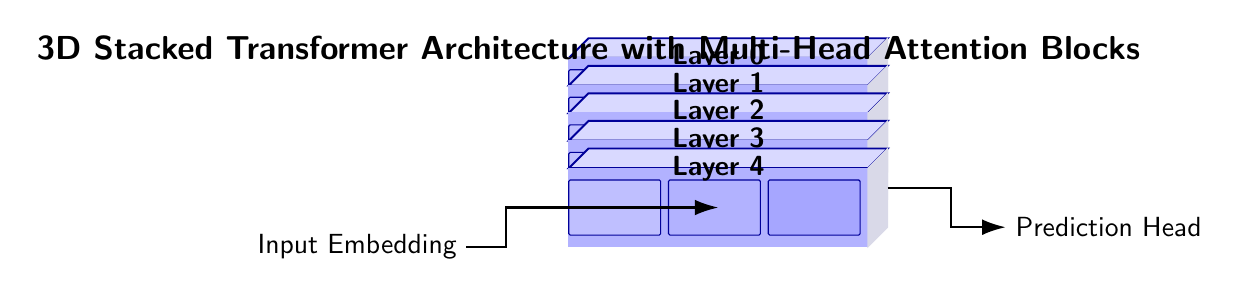
\begin{tikzpicture}[
    layerstyle/.style={
        draw=blue!60!black,
        fill=blue!15,
        line width=0.7pt
    },
    subblock/.style={
        draw=blue!60!black,
        line width=0.4pt,
        rounded corners=0.5pt
    },
    arrow/.style={
        -{Latex[length=3mm, width=2mm]},
        thick
    },
    font=\sffamily
]

% Geometry parameters
\def\w{3.8}     % layer width
\def\h{1.0}     % layer height
\def\d{0.25}    % layer depth
\def\nsubs{3}   % number of sub-blocks per layer

% Macro: draw one 3D Transformer layer with sub-blocks
\newcommand{\drawlayer}[3]{%
  % Base coordinates
  \coordinate (A) at (#1,#2);
  \coordinate (B) at ($(A)+(\w,0)$);
  \coordinate (C) at ($(B)+(\d,\d)$);
  \coordinate (D) at ($(A)+(\d,\d)$);
  \coordinate (E) at ($(A)+(0,\h)$);
  \coordinate (F) at ($(E)+(\w,0)$);
  \coordinate (G) at ($(F)+(\d,\d)$);
  \coordinate (H) at ($(E)+(\d,\d)$);

  % Layer faces
  \filldraw[layerstyle] (E) -- (F) -- (G) -- (H) -- cycle; % top
  \filldraw[blue!30!white] (A) -- (B) -- (F) -- (E) -- cycle; % front
  \filldraw[blue!40!black!15] (B) -- (C) -- (G) -- (F) -- cycle; % side

  % Sub-blocks inside the front face (Multi-Head Attention, FFN, Norm)
  \pgfmathsetmacro{\subw}{\w/\nsubs}
  \foreach \i in {0,...,\numexpr\nsubs-1} {
    \pgfmathsetmacro{\shade}{25 + 5*\i} % compute valid color blend
    \coordinate (sA) at ($(A)+(\i*\subw,0.15)$);
    \coordinate (sF) at ($(sA)+(\subw-0.1,\h-0.3)$);
    \filldraw[subblock, fill=blue!\shade!white] (sA) rectangle (sF);
  }

  % Layer label
  \node[font=\sffamily\bfseries, align=center] 
        at ($(A)!0.5!(F)+(0,0.5*\h)$) {#3};
}

% Draw stacked layers (5 layers total)
\foreach \i in {0,...,4}{
  \pgfmathsetmacro{\y}{-\i*0.35}
  \drawlayer{0}{\y}{Layer \i};
}

% Arrows and labels
\node[font=\sffamily, left=1.3cm of A] (input) {Input Embedding};
\draw[arrow] (input.east) -- ++(0.5,0) |- ($(A)!0.5!(F)$);

\node[font=\sffamily, right=1.5cm of C] (output) {Prediction Head};
\draw[arrow] ($(C)!0.5!(G)$) -- ++(0.8,0) |- (output.west);

% Title
\node[font=\sffamily\bfseries\large, above=1cm of H] 
    {3D Stacked Transformer Architecture with Multi-Head Attention Blocks};

\end{tikzpicture}
\end{document}

